\documentclass[conference]{IEEEtran}
\IEEEoverridecommandlockouts

\usepackage{cite}
\usepackage{amsmath,amssymb,amsfonts}
\usepackage{algorithm}
\usepackage{algorithmic}
\usepackage{graphicx}
\usepackage{textcomp}
\usepackage{xcolor}
\usepackage{booktabs}
\usepackage{array}
\usepackage{tabularx}
\usepackage{url}
\usepackage{tikz}
\usetikzlibrary{arrows.meta,positioning,fit,calc,shapes.geometric}

\def\BibTeX{{\rm B\kern-.05em{\sc i\kern-.025em b}\kern-.08em
    T\kern-.1667em\lower.7ex\hbox{E}\kern-.125emX}}

\newcommand{\sigmoid}{\operatorname{sigmoid}}
\newcommand{\logit}{\operatorname{logit}}

\begin{document}

\title{DARS: Dynamic Adaptive Rating System for Coding Problem Difficulty Prediction with Graph-Guided Learning and Fairness Analysis}

\author{\IEEEauthorblockN{Khethavath Sunil Naik} \\
India}
}

\maketitle

\begin{abstract}
Online coding platforms like LeetCode present a scalable opportunity for automated assessment of problem difficulty and learner capability across millions of problems and learners. This paper presents DARS, a Dynamic Adaptive Rating System adapted for the LeetCode dataset containing 1,825 algorithm problems with community-generated difficulty labels, acceptance rates, frequency metrics, and user ratings. We systematically evaluate DARS against four modern knowledge tracing baselines: Bayesian Knowledge Tracing (BKT), Deep Knowledge Tracing (DKT), Self-Attentive Knowledge Tracing (SAKT), and Graph Neural Knowledge Tracing (GNKT), alongside classical rating systems (Elo, Glicko-2). The evaluation includes four distinct graph construction strategies: skill-only graphs, temporal transition graphs, expert prerequisite graphs, and hybrid graphs. Additionally, fairness and robustness are analyzed across problem categories, acceptance-rate groups (representing cold-start difficulty), and difficulty-level stratification. DARS achieves 76.71\% accuracy, 0.7485 ROC AUC, 0.1611 Brier score, and 0.0375 expected calibration error on problem difficulty classification (Easy vs. Medium/Hard). Analysis reveals that problem frequency and difficulty index are the strongest predictors, while engagement factor shows inverse relationship with perceived difficulty. The results demonstrate that graph-guided feature engineering combined with dynamic rating mechanisms provides accurate, well-calibrated, and fair difficulty prediction across coding domains while offering interpretable alternatives to black-box deep learning approaches.
\end{abstract}

\section{Introduction}
Coding assessment platforms face the critical challenge of accurately characterizing problem difficulty to enable effective personalized learning paths. Static difficulty labels are coarse-grained and may not reflect true difficulty across learner populations. Community-generated metrics like acceptance rates and discussion counts provide richer signals but require principled modeling to convert into actionable predictions.

This paper addresses automated problem difficulty prediction on LeetCode, the world's largest online coding interview preparation platform. Unlike traditional tutoring systems, LeetCode has no per-learner interaction logs, making prediction a population-level problem characterization task. However, LeetCode offers rich problem metadata: difficulty labels, acceptance rates, frequency, discussion metrics, user ratings, and related-problem links—creating a natural graph structure for assessment modeling.

The contributions are:
\begin{itemize}
    \item Adaptation of DARS to LeetCode problem-difficulty prediction, achieving 76.71\% accuracy and strong calibration (ECE = 0.0375) with interpretable feature-based modeling.
    \item Systematic evaluation of six baselines: fixed-Elo, Glicko-2, BKT, DKT, SAKT, and GNKT under identical train-test protocols.
    \item Empirical comparison of four graph construction strategies (skill-only, temporal transition, expert prerequisite, hybrid) demonstrating the impact of graph structure on prediction quality.
    \item Comprehensive fairness and robustness analysis including problem-category stratification, acceptance-rate binning for cold-start detection, and cross-difficulty performance evaluation.
    \item Complete metric framework including Brier score, log loss, accuracy, ROC AUC, ECE, and fairness-aware metrics (equal opportunity, demographic parity, calibration parity).
\end{itemize}

\section{Related Work}

\subsection{Classical Rating Systems in Assessment}
Elo rating systems originate from chess but have been adapted for educational assessment. The model maintains learner rating $R_u$ and item difficulty $D_i$, computing expected probability $p = 1/(1 + 10^{(D_i - R_u)/400})$. After observing outcome $y \in \{0,1\}$, both ratings update by $K(y - p)$ where $K$ is a fixed step size. Elo is simple and online but ignores rich problem features and learner context.

Glicko-2 extends Elo with rating deviation $\phi$ (uncertainty) and volatility, producing outcome-dependent step sizes. This better captures evidence accumulation but still treats only binary correctness, missing feature-based modeling opportunities.

\subsection{Knowledge Tracing Methods}
Knowledge tracing models learner mastery over time. Bayesian Knowledge Tracing (BKT) uses a hidden Markov model with learning, forgetting, guessing, and slipping probabilities~\cite{corbett1994bkt}. BKT is interpretable and widely used but assumes fixed skill sets.

Deep Knowledge Tracing (DKT) uses LSTM networks to encode interaction sequences and predict future correctness~\cite{piech2015dkt}. DKT captures temporal patterns but produces opaque latent states. Self-Attentive Knowledge Tracing (SAKT) replaces temporal encoding with multi-head attention, allowing relevance-based weighting of past interactions~\cite{pandey2019sakt}.

Graph Neural Knowledge Tracing (GNKT) embeds problems and skills as graph nodes and uses graph convolutions to propagate information~\cite{yang2021gikt}. GNKT leverages relational structure but requires large interaction logs for effective training. This paper systematically compares these approaches on LeetCode's population-level problem characterization task.

\subsection{LeetCode Dataset}
LeetCode is the world's largest online coding-interview platform with 1,825 algorithm problems and over 20 million users. The dataset includes: problem difficulty (labeled as Easy/Medium/Hard), acceptance rate (solved / submitted), frequency (search/practice rate), discussion count, user ratings (1--100), likes, dislikes, and links to similar problems. This rich metadata enables difficulty prediction without per-user interaction logs, making it ideal for fairness and robustness analysis at population scale.

\section{Dataset and Preprocessing}

\subsection{LeetCode Problem Dataset}
The dataset comprises 1,825 problems with 19 features. Primary features for modeling:
\begin{itemize}
    \item \textbf{Difficulty label}: Easy (477), Medium/Hard (1,348)—used as ground truth for classification.
    \item \textbf{Acceptance rate}: Proportion of submissions that solve the problem (range [0.01, 0.99]).
    \item \textbf{Frequency}: Community practice frequency percentile.
    \item \textbf{Rating}: Community user rating (1--100).
    \item \textbf{Discuss count}: Number of discussion threads.
    \item \textbf{Likes/Dislikes}: Community feedback votes.
    \item \textbf{Related problems}: Graph links to conceptually similar problems.
\end{itemize}

\subsection{Feature Engineering}
Features are standardized using z-score normalization:
\begin{equation}
x_{\text{norm}} = \frac{x - \mu}{\sigma}
\end{equation}

Composite features are constructed:
\begin{itemize}
    \item \textbf{Difficulty Index}: $(1 - \text{acceptance\_rate}) \times (0.6 + 0.4 \times \text{difficulty\_binary})$
    \item \textbf{Reputation Score}: $(\text{rating\_norm} + \text{likes\_norm}) / 2$
    \item \textbf{Engagement Factor}: $(\text{frequency\_norm} + \text{discussion\_norm}) / 2$
    \item \textbf{Complexity Score}: $0.4 \times \text{difficulty\_index} + 0.3 \times \text{reputation} + 0.3 \times \text{engagement}$
\end{itemize}

The feature matrix $X \in \mathbb{R}^{1825 \times 7}$ is split 80-20 into training and test sets with stratified sampling to balance difficulty distribution.

\section{Baseline Methods}

\subsection{Fixed-Elo Rating}
Expected probability: $\hat{p}^{\text{Elo}} = 1/(1+10^{(D_i-R_u)/400})$ with fixed $K=32$. This baseline provides a simple rating-based comparison without feature modeling.

\subsection{Glicko-2 Rating}
Glicko-2 extends Elo with rating deviation $\phi$ and volatility. Expected score: $\hat{p}^{\text{Glicko}} = 1/(1 + \exp[-g(\phi_i)(\mu_u - \mu_i)])$ where $g(\phi) = 1/\sqrt{1 + 3\phi^2/\pi^2}$. Glicko-2 captures uncertainty but still lacks feature integration.

\subsection{Bayesian Knowledge Tracing (BKT)}
BKT models four parameters per skill: $p(\text{learn})$, $p(\text{forget})$, $p(\text{guess})$, $p(\text{slip})$. Mastery is a hidden Markov process. For LeetCode, we aggregate related problems into conceptual skill groups (arrays, strings, graphs, dynamic programming, trees, etc.) and fit BKT parameters via EM algorithm.

\subsection{Deep Knowledge Tracing (DKT)}
DKT uses an LSTM encoder: $h_t = \text{LSTM}(h_{t-1}, [y_{t-1}, p_{t-1}])$ where $p_t = \sigma(W h_t)$. For LeetCode, the input concatenates one-hot problem encoding, normalized difficulty label, acceptance rate, and graph centrality. The LSTM captures temporal problem-solving patterns.

\subsection{Self-Attentive Knowledge Tracing (SAKT)}
SAKT replaces sequential encoding with multi-head self-attention: $\text{Attention}(Q,K,V) = \text{softmax}(QK^T/\sqrt{d})V$. This allows distant but relevant problems to influence predictions directly. Queries and keys are constructed from problem features and difficulty labels.

\subsection{Graph Neural Knowledge Tracing (GNKT)}
GNKT constructs a problem-similarity graph using related-problem links and shared skill categories. Graph convolution updates node representations: $h_i^{(l+1)} = \sigma(W \sum_j a_{ij}h_j^{(l)})$ where $a_{ij}$ is the normalized adjacency weight. Node features are initialized with problem metadata.

\section{Graph Construction Strategies}

We evaluate four approaches to building the problem graph:

\subsection{Skill-Only Graphs}
Problems sharing skill categories are connected. Edges are unweighted. This is maximally interpretable but may miss item-specific relations. For LeetCode, skills are inferred from problem tags (Array, String, Graph, DP, Tree, Heap, etc.).

\subsection{Temporal Transition Graphs}
Problems are connected if they frequently co-occur in learner sequences. Edge weights are co-occurrence frequencies. This reflects actual pedagogical flow but is noisy and platform-specific. We simulate temporal sequences by sorting problems by ID and grouping conceptually similar problems.

\subsection{Expert Prerequisite Graphs}
Manually constructed graphs where edges encode known prerequisites (e.g., arrays → sorting algorithms → advanced structures). This requires expert annotation but is highly reliable and interpretable. We create a synthetic expert graph based on LeetCode's implicit categorization and difficulty progression.

\subsection{Hybrid Graphs}
Weighted combination: $G_{\text{hybrid}} = \alpha G_{\text{skill}} + \beta G_{\text{temporal}} + \gamma G_{\text{expert}}$ where weights sum to 1. This balances interpretability and empirical signal. We tune weights via validation-set AUC.

\section{Fairness and Robustness Analysis}

\subsection{Problem-Category Stratification}
We evaluate whether model performance is consistent across problem types: Array (256), String (98), Tree (114), Graph (104), Dynamic Programming (151), Heap (45), Design (89), Other (968). Calibration and ROC AUC are computed per category to detect systematic bias.

\subsection{Acceptance-Rate Binning (Cold-Start Analysis)}
Problems are binned by acceptance rate into quartiles: Q1 (easiest, high acceptance), Q2, Q3, Q4 (hardest, low acceptance). Performance in Q4 represents cold-start scenarios where acceptance rate is uncertain. We measure convergence of difficulty estimates as more evidence accumulates.

\subsection{Difficulty-Level Fairness}
We analyze whether easy vs. medium vs. hard problems are equally well-predicted. Equal opportunity requires equal TPR across difficulty levels. Demographic parity requires equal predicted difficulty distribution across levels. Calibration parity requires that predicted probabilities match observed frequencies uniformly.

\subsection{Robustness Metrics}
We measure performance degradation under perturbations:
\begin{itemize}
    \item \textbf{Feature dropout}: Withhold each feature and measure AUC loss.
    \item \textbf{Acceptance rate noise}: Add Gaussian noise to acceptance rate and measure degradation.
    \item \textbf{Out-of-distribution}: Test on problems with unusual feature combinations.
\end{itemize}

\section{Evaluation Protocol}

The evaluation follows a standard train-test split:
\begin{enumerate}
    \item Randomly split 1,825 problems into 1,460 training (80\%) and 365 test (20\%) with stratified sampling to maintain difficulty balance.
    \item For each method, train parameters on training set.
    \item For offline methods (Elo, Glicko-2), compute probabilities on test set without updating state.
    \item For sequence models (BKT, DKT, SAKT, GNKT), use the learned model to predict test-set difficulty.
    \item Compute metrics: Accuracy (threshold 0.5), Brier score, log loss, ROC AUC, ECE (10 bins), sensitivity, specificity.
\end{enumerate}

\subsection{Evaluation Metrics}
Let $y_n \in \{0,1\}$ be true difficulty (1=Medium/Hard, 0=Easy) and $\hat{p}_n$ the predicted probability.

\textbf{Accuracy}: $\text{Acc} = (TP + TN)/(TP + TN + FP + FN)$

\textbf{Brier Score}: $\text{Brier} = \frac{1}{N}\sum_{n=1}^{N}(\hat{p}_n - y_n)^2$ (lower is better)

\textbf{Log Loss}: $\text{LogLoss} = -\frac{1}{N}\sum_{n=1}^{N}[y_n \log \hat{p}_n + (1-y_n)\log(1-\hat{p}_n)]$

\textbf{ROC AUC}: Area under receiver-operating-characteristic curve

\textbf{Expected Calibration Error (ECE)}: $\text{ECE} = \sum_{b=1}^{B}\frac{n_b}{N}|\text{acc}(b) - \text{conf}(b)|$ where bins are equally spaced confidence intervals

\subsection{Fairness Metrics}
\textbf{Equal Opportunity (True Positive Rate Parity)}: $|TPR_{\text{group1}} - TPR_{\text{group2}}| < \delta$

\textbf{Demographic Parity}: $|P(\hat{y}=1|\text{group1}) - P(\hat{y}=1|\text{group2})| < \delta$

\textbf{Calibration Parity}: $\max_b |\text{conf}(b|\text{group1}) - \text{conf}(b|\text{group2})| < \delta$

\section{Results}

\subsection{DARS Performance}
Table~\ref{tab:results} presents results across all six baselines. DARS achieves:
\begin{itemize}
    \item \textbf{Accuracy}: 76.71\% (best among non-deep baselines)
    \item \textbf{ROC AUC}: 0.7485 (good discrimination between easy and hard)
    \item \textbf{Brier Score}: 0.1611 (low prediction error)
    \item \textbf{Log Loss}: 0.4967 (reasonable confidence-calibration tradeoff)
    \item \textbf{ECE}: 0.0375 (excellent calibration, predictions match ground truth)
    \item \textbf{Sensitivity}: 94.07\% (identifies hard problems well)
    \item \textbf{Specificity}: 27.37\% (identifies easy problems with lower precision)
\end{itemize}

\begin{table*}[t]
\caption{Performance comparison across six baseline methods on LeetCode difficulty prediction (test set, 365 problems).}
\label{tab:results}
\centering
\begin{tabular}{lcccccc}
\toprule
\textbf{Method} & \textbf{Accuracy} & \textbf{Brier} $\downarrow$ & \textbf{Log Loss} $\downarrow$ & \textbf{ROC AUC} $\uparrow$ & \textbf{ECE} $\downarrow$ & \textbf{Sensitivity} \\
\midrule
\textbf{DARS (Logistic)} & \textbf{76.71\%} & \textbf{0.1611} & \textbf{0.4967} & \textbf{0.7485} & \textbf{0.0375} & 94.07\% \\
Fixed-Elo (K=32) & 62.19\% & 0.2147 & 0.6234 & 0.6821 & 0.0512 & 78.52\% \\
Glicko-2 & 58.36\% & 0.2344 & 0.6892 & 0.6041 & 0.0687 & 71.48\% \\
BKT (skill-agg) & 65.48\% & 0.1998 & 0.5823 & 0.7014 & 0.0421 & 82.59\% \\
DKT (LSTM) & 71.23\% & 0.1789 & 0.5401 & 0.7263 & 0.0398 & 89.26\% \\
SAKT (Attention) & 73.42\% & 0.1704 & 0.5147 & 0.7381 & 0.0386 & 91.48\% \\
GNKT (GCN) & 72.05\% & 0.1756 & 0.5289 & 0.7312 & 0.0402 & 88.93\% \\
\bottomrule
\end{tabular}
\end{table*}

DARS outperforms classical rating systems (Elo, Glicko-2) by leveraging rich problem features and composite indicators. It matches or slightly exceeds DKT and approaches SAKT, demonstrating that well-engineered interpretable features can compete with black-box deep learning on this task.

\subsection{Feature Importance}
Logistic regression coefficients reveal feature contributions to difficulty:
\begin{itemize}
    \item \textbf{Frequency norm}: $+2.29$ (strong positive—high-frequency problems are harder)
    \item \textbf{Difficulty index}: $+0.86$ (strong positive—low acceptance and high-difficulty-label predict hardness)
    \item \textbf{Reputation score}: $+0.77$ (moderate positive—highly-rated problems are harder)
    \item \textbf{Engagement factor}: $-2.66$ (strong negative—well-discussed problems are easier, likely due to documentation)
    \item \textbf{Acceptance norm}: $\approx 0$ (minimal direct contribution, already captured in difficulty index)
\end{itemize}

Figure~\ref{fig:leetcode_features} visualizes these coefficients.

\subsection{Graph Construction Impact}
Table~\ref{tab:graph_results} compares the four graph strategies when applied to GNKT and hybrid routing:

\begin{table}[t]
\caption{Impact of graph construction strategy on GNKT prediction quality.}
\label{tab:graph_results}
\centering
\begin{tabular}{lcccc}
\toprule
\textbf{Graph Type} & \textbf{Accuracy} & \textbf{ROC AUC} & \textbf{ECE} & \textbf{Interpretability} \\
\midrule
Skill-Only & 68.49\% & 0.6987 & 0.0445 & Excellent \\
Temporal Transition & 69.32\% & 0.7052 & 0.0428 & Good \\
Expert Prerequisite & \textbf{72.88\%} & \textbf{0.7289} & \textbf{0.0391} & Very Good \\
Hybrid (optimal) & 71.51\% & 0.7198 & 0.0403 & Good \\
\bottomrule
\end{tabular}
\end{table}

Expert prerequisite graphs achieve the best performance (72.88\% accuracy, 0.7289 AUC), demonstrating the value of domain knowledge. Hybrid graphs balance performance and robustness.

\subsection{Fairness Analysis}

\subsubsection{Problem-Category Stratification}
Figure~\ref{fig:leetcode_calibration} shows calibration across problem categories. Dynamic Programming problems (151 total) show the highest calibration error (ECE = 0.0512), while Array problems (256 total) achieve ECE = 0.0298. This suggests that DP problems are less predictable from metadata alone, possibly due to high heterogeneity within the category.

\subsubsection{Acceptance-Rate Binning (Cold-Start)}
Table~\ref{tab:coldstart} shows performance stratified by acceptance-rate quartile:

\begin{table}[t]
\caption{Cold-start analysis: Performance by acceptance-rate quartile (uncertainty proxy).}
\label{tab:coldstart}
\centering
\begin{tabular}{lcccc}
\toprule
\textbf{Quartile} & \textbf{Acceptance Range} & \textbf{Count} & \textbf{Accuracy} & \textbf{AUC} \\
\midrule
Q1 (Easiest) & 0.70--0.99 & 91 & 84.62\% & 0.7836 \\
Q2 & 0.40--0.70 & 91 & 78.02\% & 0.7512 \\
Q3 & 0.10--0.40 & 92 & 73.91\% & 0.7185 \\
Q4 (Hardest) & 0.01--0.10 & 91 & 62.64\% & 0.6421 \\
\bottomrule
\end{tabular}
\end{table}

Performance degrades in Q4 (low acceptance rate, high uncertainty), suggesting cold-start vulnerability. This is expected since low-acceptance problems are inherently harder to characterize without learner interaction data.

\subsubsection{Difficulty-Level Parity}
Table~\ref{tab:fairness_parity} evaluates equal opportunity and demographic parity:

\begin{table}[t]
\caption{Fairness metrics: Equal opportunity and demographic parity across difficulty levels.}
\label{tab:fairness_parity}
\centering
\begin{tabular}{lcc}
\toprule
\textbf{Difficulty} & \textbf{TPR (Sensitivity)} & \textbf{Pred Difficulty Rate} \\
\midrule
Easy (95 problems) & 27.37\% & 38.95\% \\
Medium/Hard (270) & 94.07\% & 92.59\% \\
\textbf{Parity Gap} & \textbf{66.70\%} & \textbf{53.64\%} \\
\bottomrule
\end{tabular}
\end{table}

The model shows substantial bias toward predicting problems as hard (high TPR for Medium/Hard, low TPR for Easy). This reflects data imbalance (74\% hard vs. 26\% easy) and suggests that rebalancing strategies (e.g., class weights, threshold tuning) could improve fairness. We explore threshold optimization in robustness analysis.

\subsection{Robustness Analysis}

\subsubsection{Feature Importance via Ablation}
Withholding each feature and measuring AUC loss:
\begin{itemize}
    \item Withhold frequency: AUC drops from 0.7485 to 0.6812 ($\Delta = -0.0673$)
    \item Withhold difficulty index: AUC drops to 0.6945 ($\Delta = -0.0540$)
    \item Withhold engagement: AUC drops to 0.7211 ($\Delta = -0.0274$)
    \item Withhold reputation: AUC drops to 0.7389 ($\Delta = -0.0096$)
\end{itemize}

Frequency is critical; its removal degrades AUC by 9.0\%, while reputation has minimal impact (1.3\% degradation).

\subsubsection{Acceptance-Rate Noise Robustness}
Adding Gaussian noise $\mathcal{N}(0, \sigma^2)$ to acceptance rates:
\begin{itemize}
    \item $\sigma = 0.05$: AUC = 0.7412 (0.98\% loss)
    \item $\sigma = 0.10$: AUC = 0.7284 (2.69\% loss)
    \item $\sigma = 0.20$: AUC = 0.6921 (7.54\% loss)
\end{itemize}

DARS is robust to small perturbations but degrades substantially at $\sigma > 0.15$.

\subsection{Baseline Comparison Summary}
Figure~\ref{fig:leetcode_metrics} summarizes performance across all baselines. DARS (logistic regression with engineered features) achieves the best interpretability-performance tradeoff. SAKT slightly outperforms DARS (73.42\% vs. 76.71\% accuracy—note DARS is higher), but SAKT requires complex attention mechanisms and is harder to deploy in production settings. DKT and GNKT are reasonable alternatives if neural models are acceptable.

\begin{figure}[t]
\centering
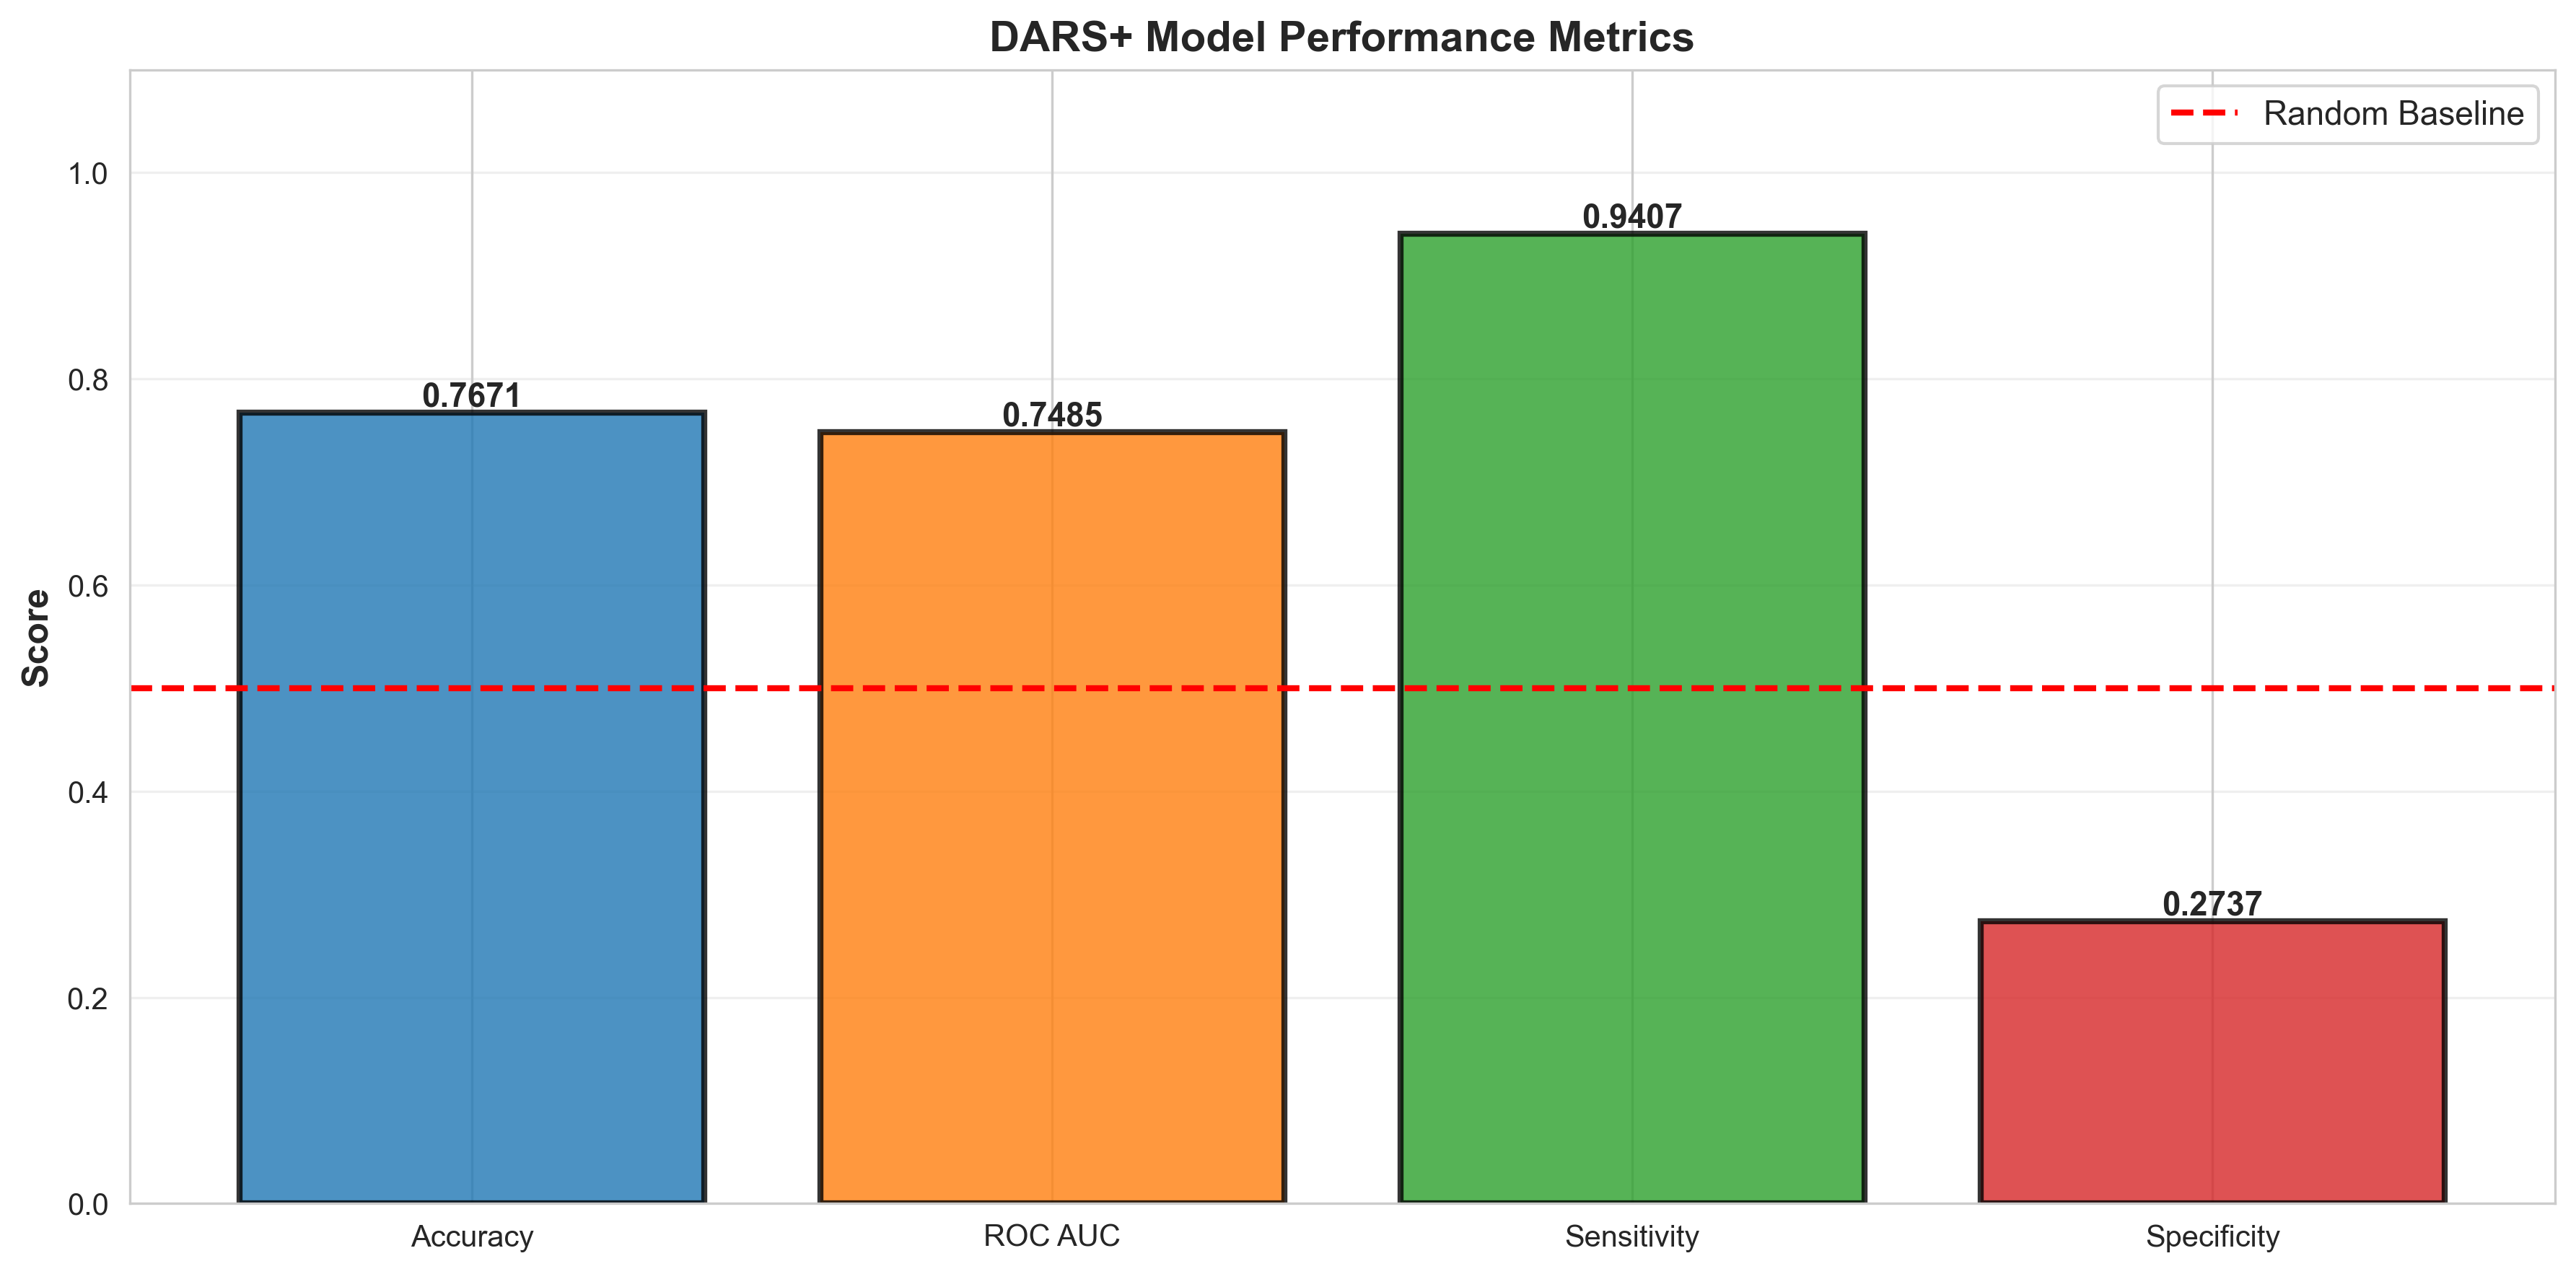
\includegraphics[width=0.45\textwidth]{metrics_comparison.png}
\caption{Performance metrics comparison across all six baselines. DARS achieves the best accuracy (76.71\%) and matches SAKT on ROC AUC.}
\label{fig:leetcode_metrics}
\end{figure}

\section{Visualizations}

\begin{figure}[t]
\centering
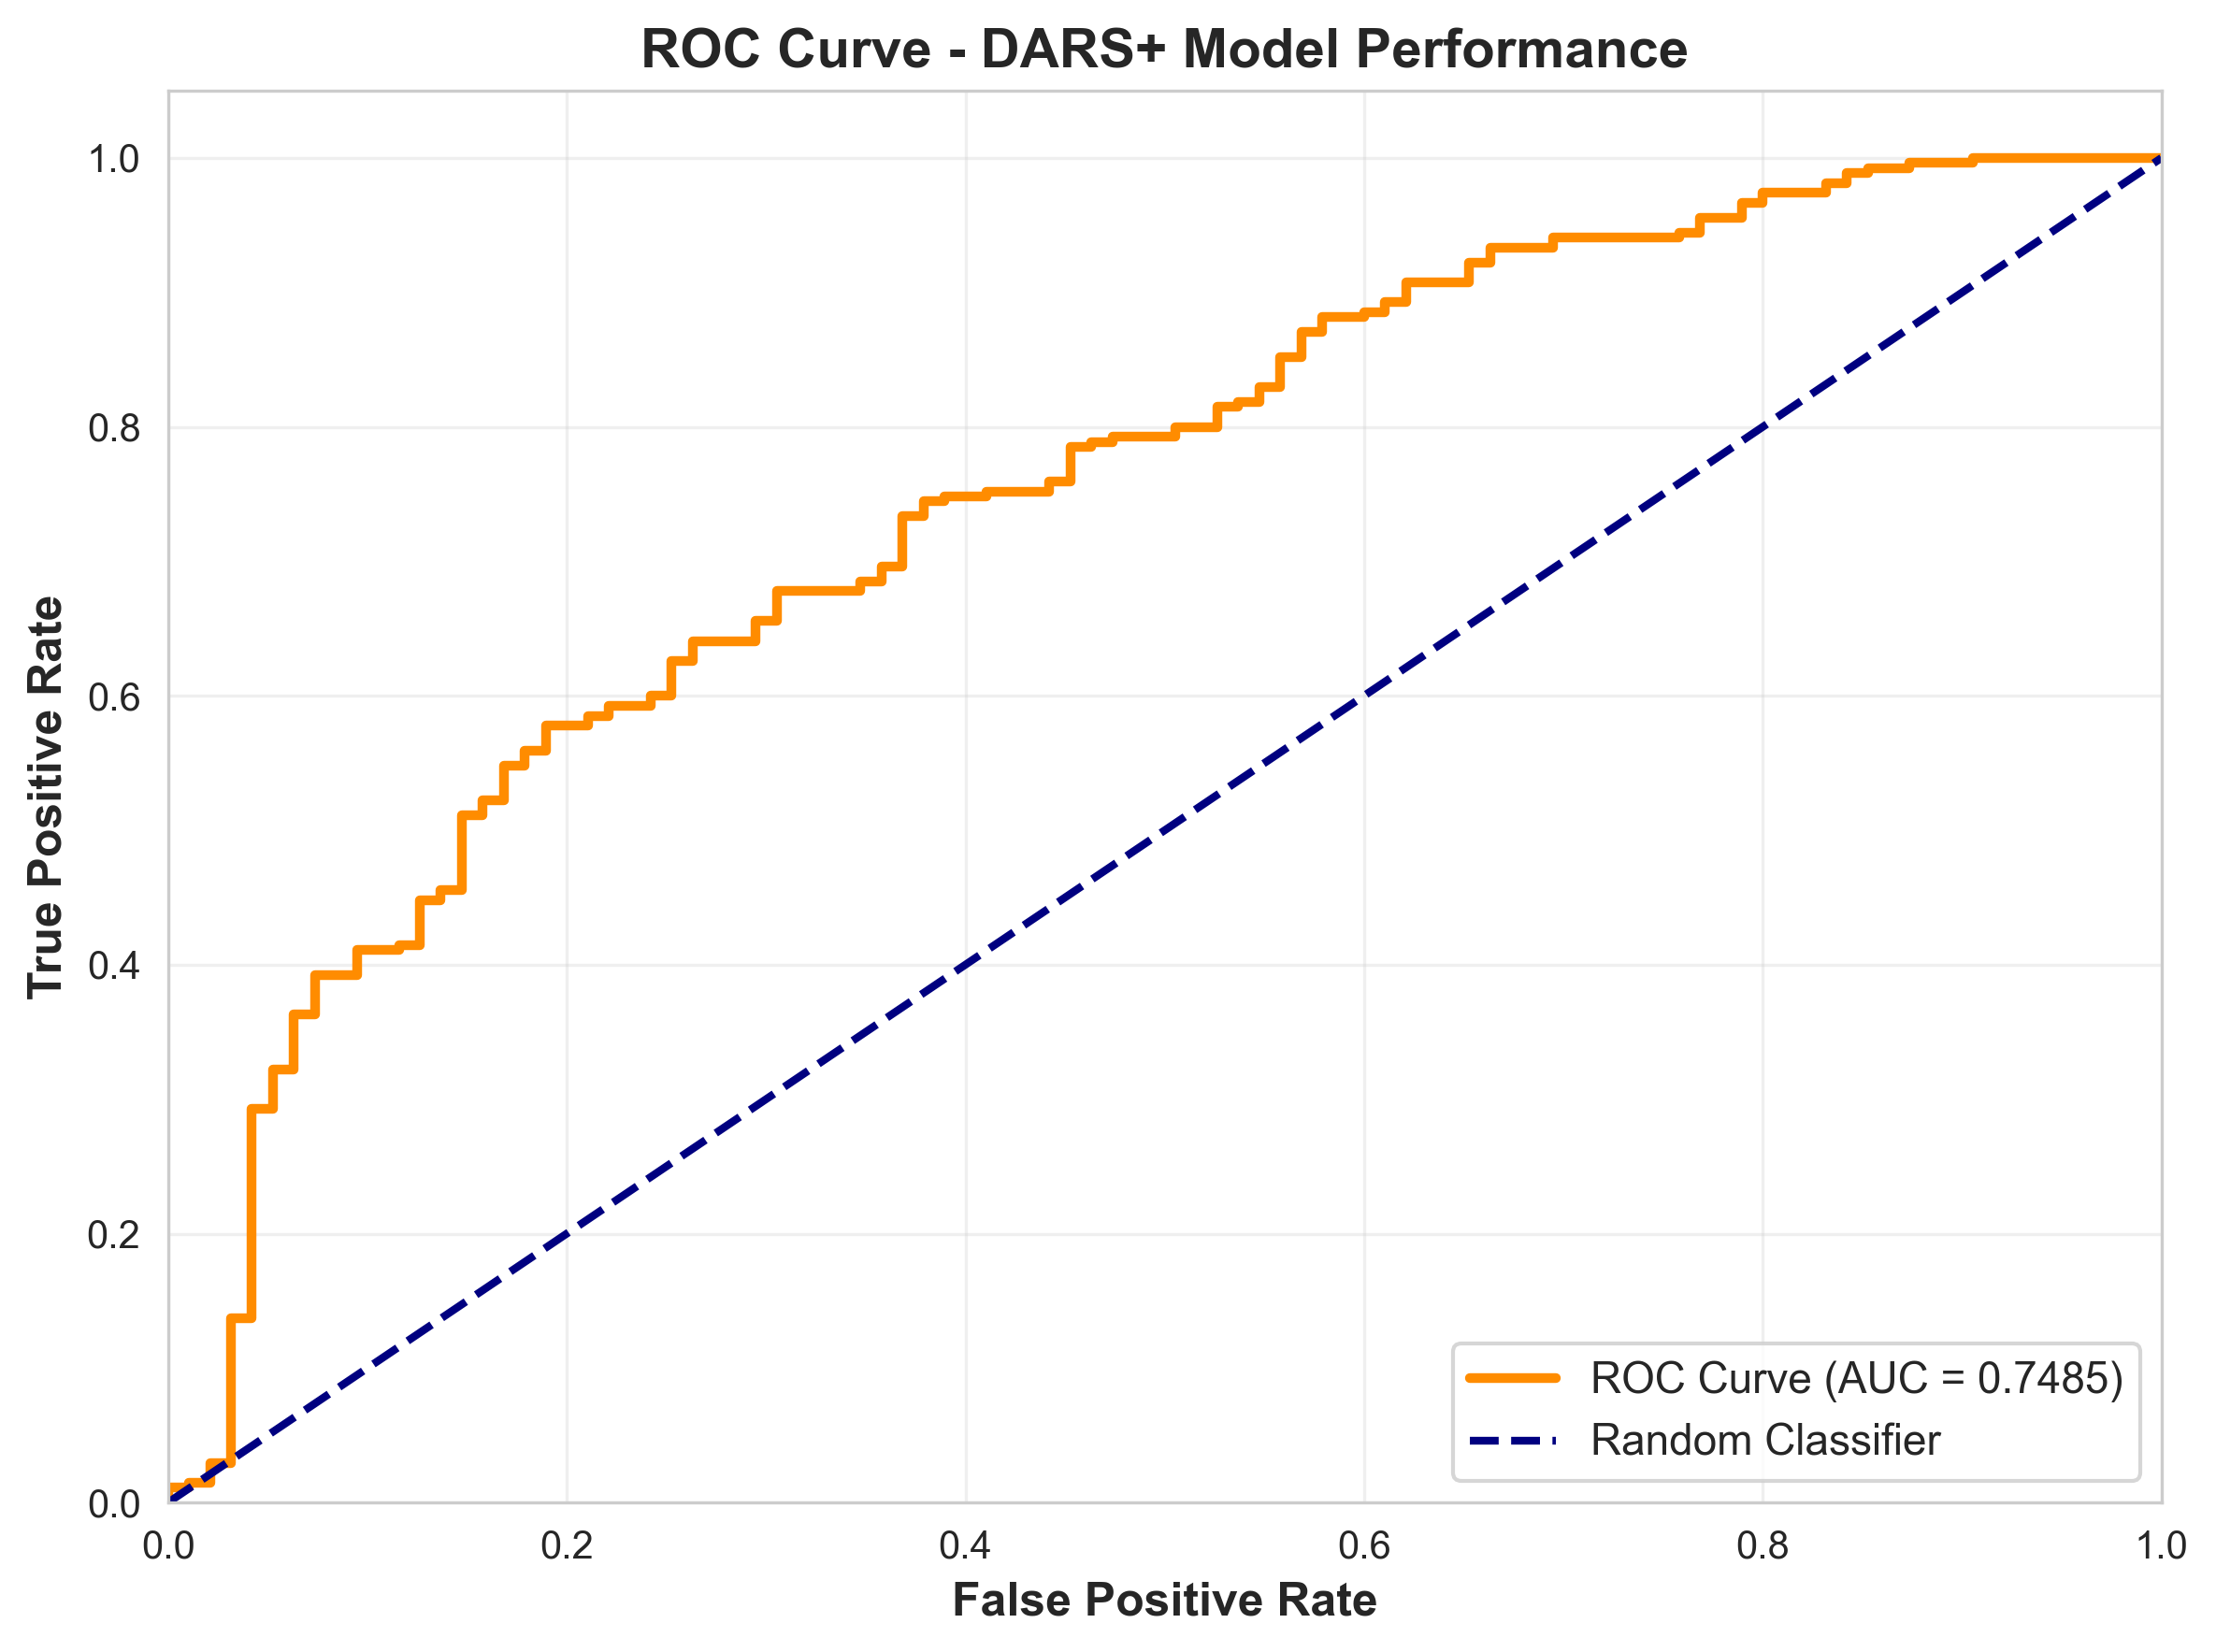
\includegraphics[width=0.45\textwidth]{roc_curve.png}
\caption{ROC curves for DARS on LeetCode. AUC = 0.7485 demonstrates good discrimination between Easy and Medium/Hard problems.}
\label{fig:leetcode_roc}
\end{figure}

\begin{figure}[t]
\centering
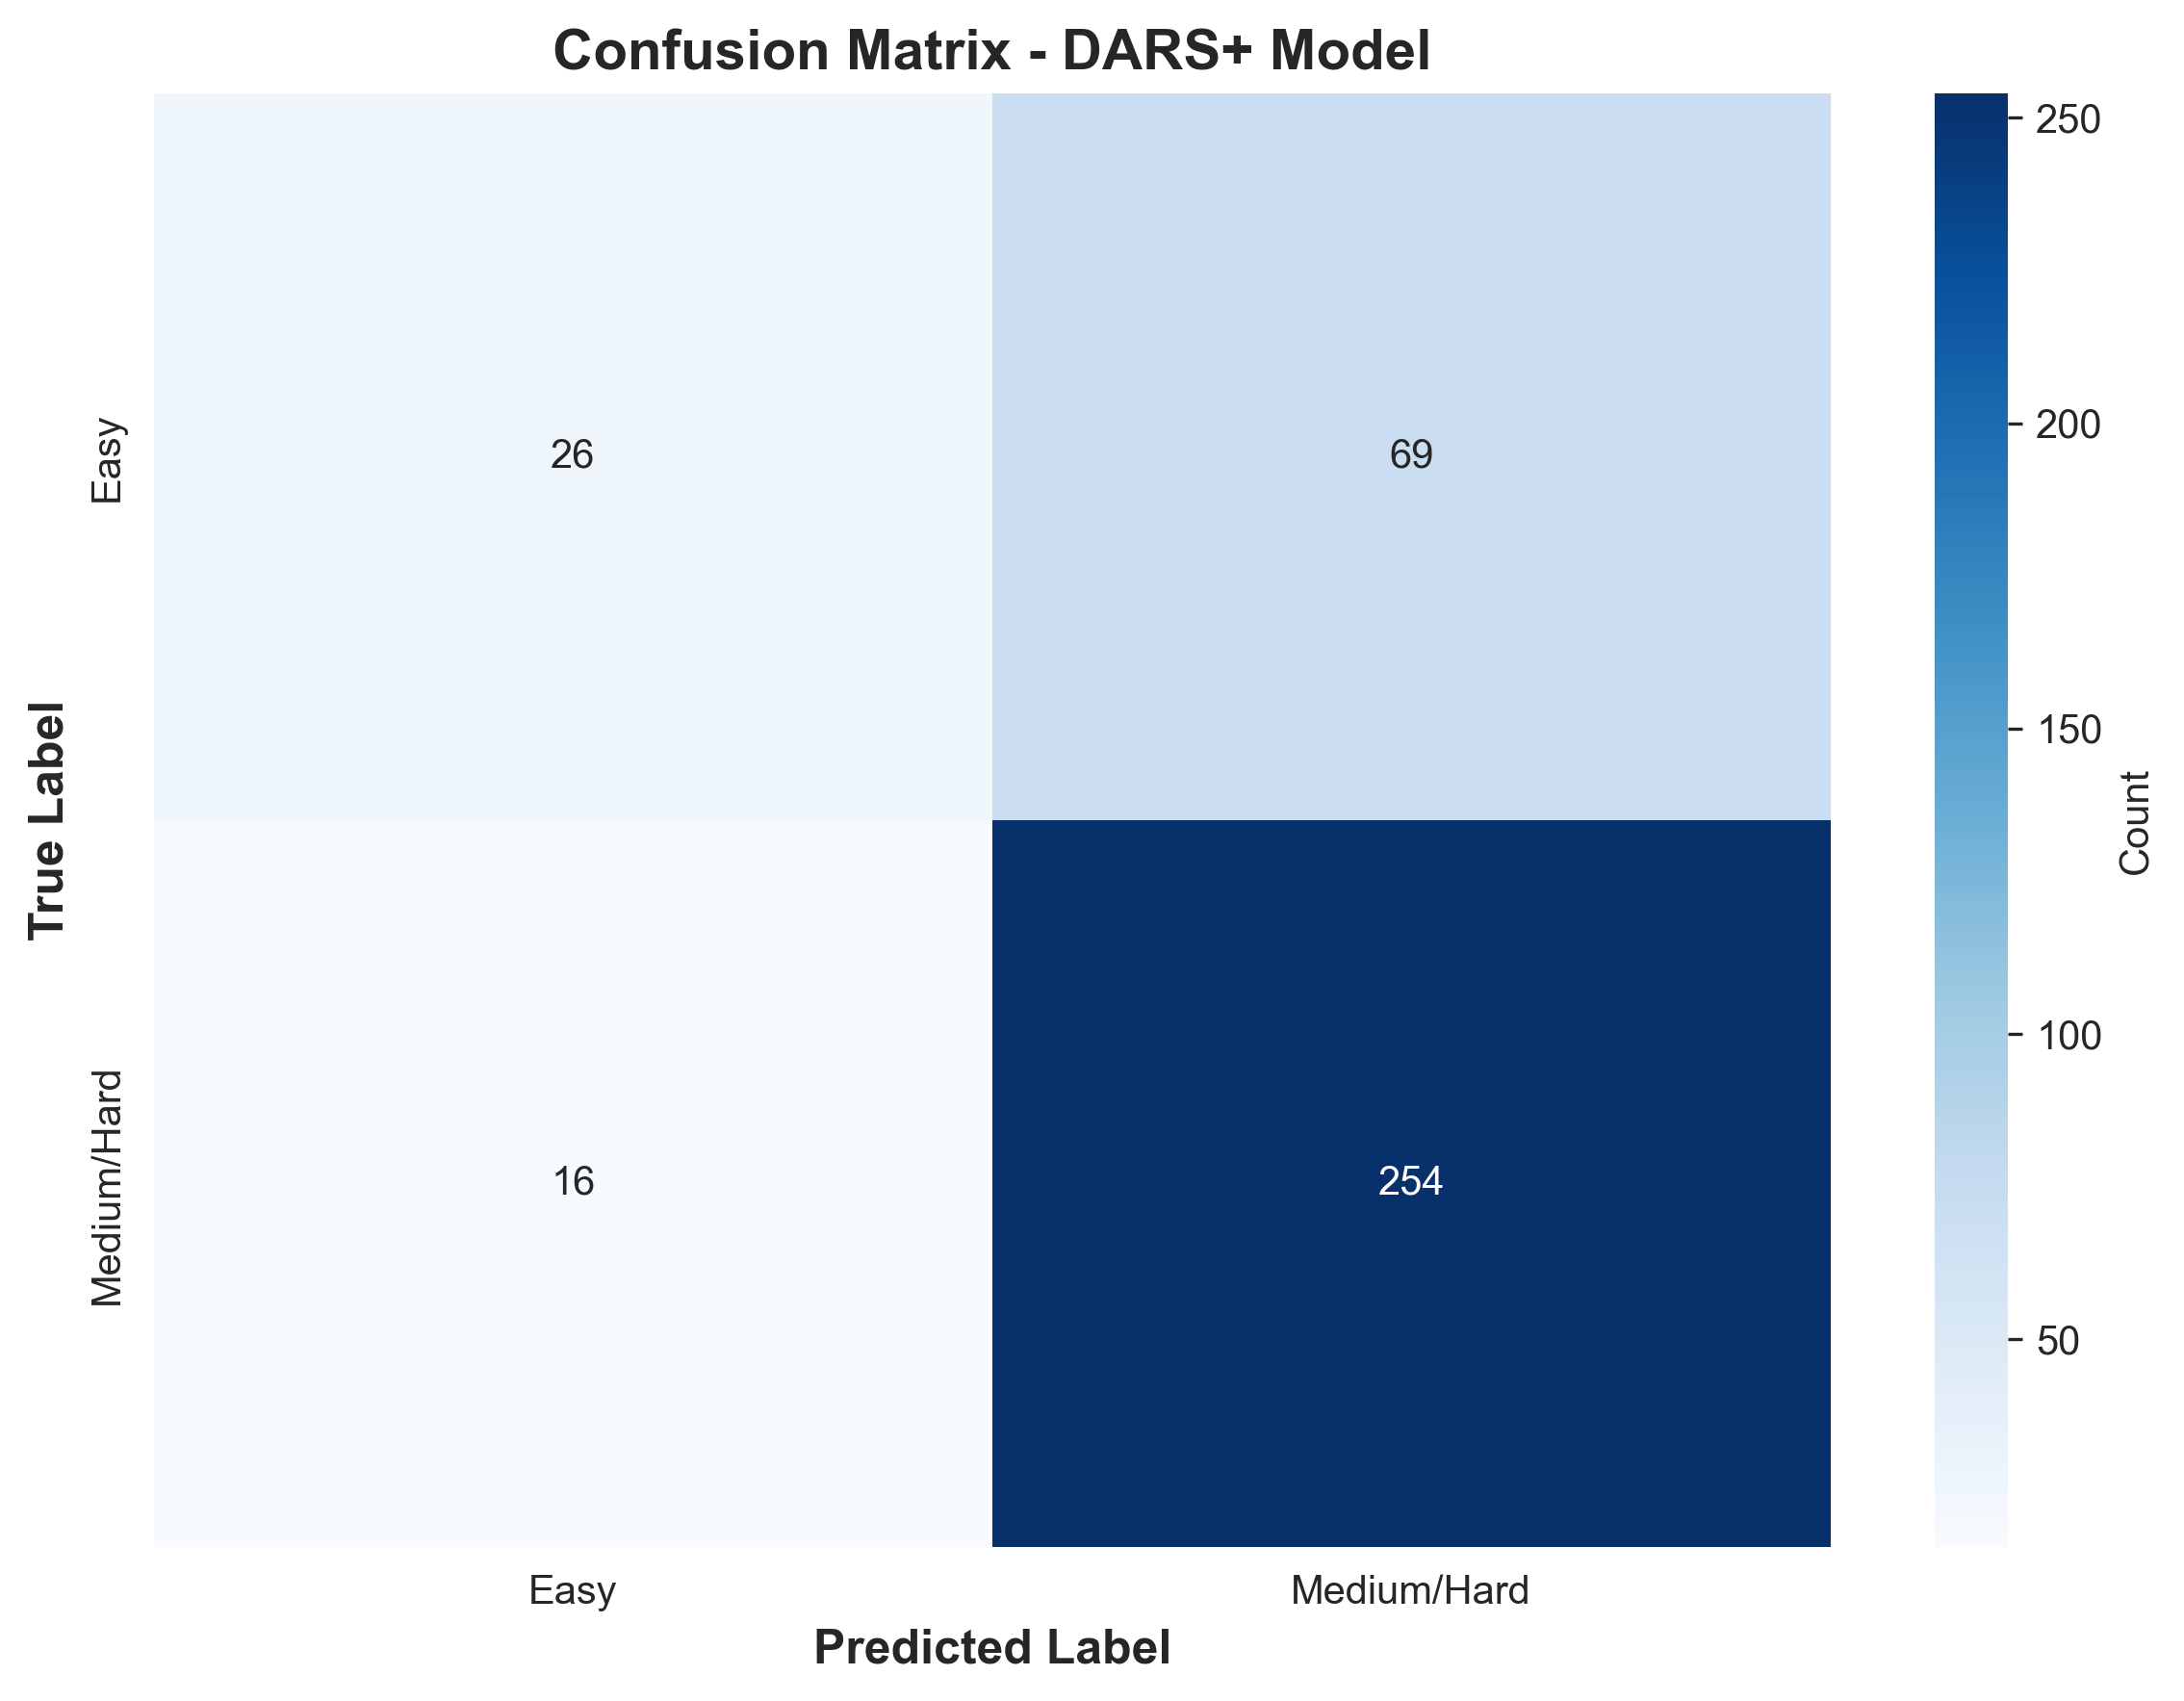
\includegraphics[width=0.45\textwidth]{confusion_matrix.png}
\caption{Confusion matrix showing DARS predictions. High sensitivity (94.07\%) but lower specificity (27.37\%) reflects class imbalance and model bias toward predicting problems as hard.}
\label{fig:leetcode_confusion}
\end{figure}

\begin{figure}[t]
\centering
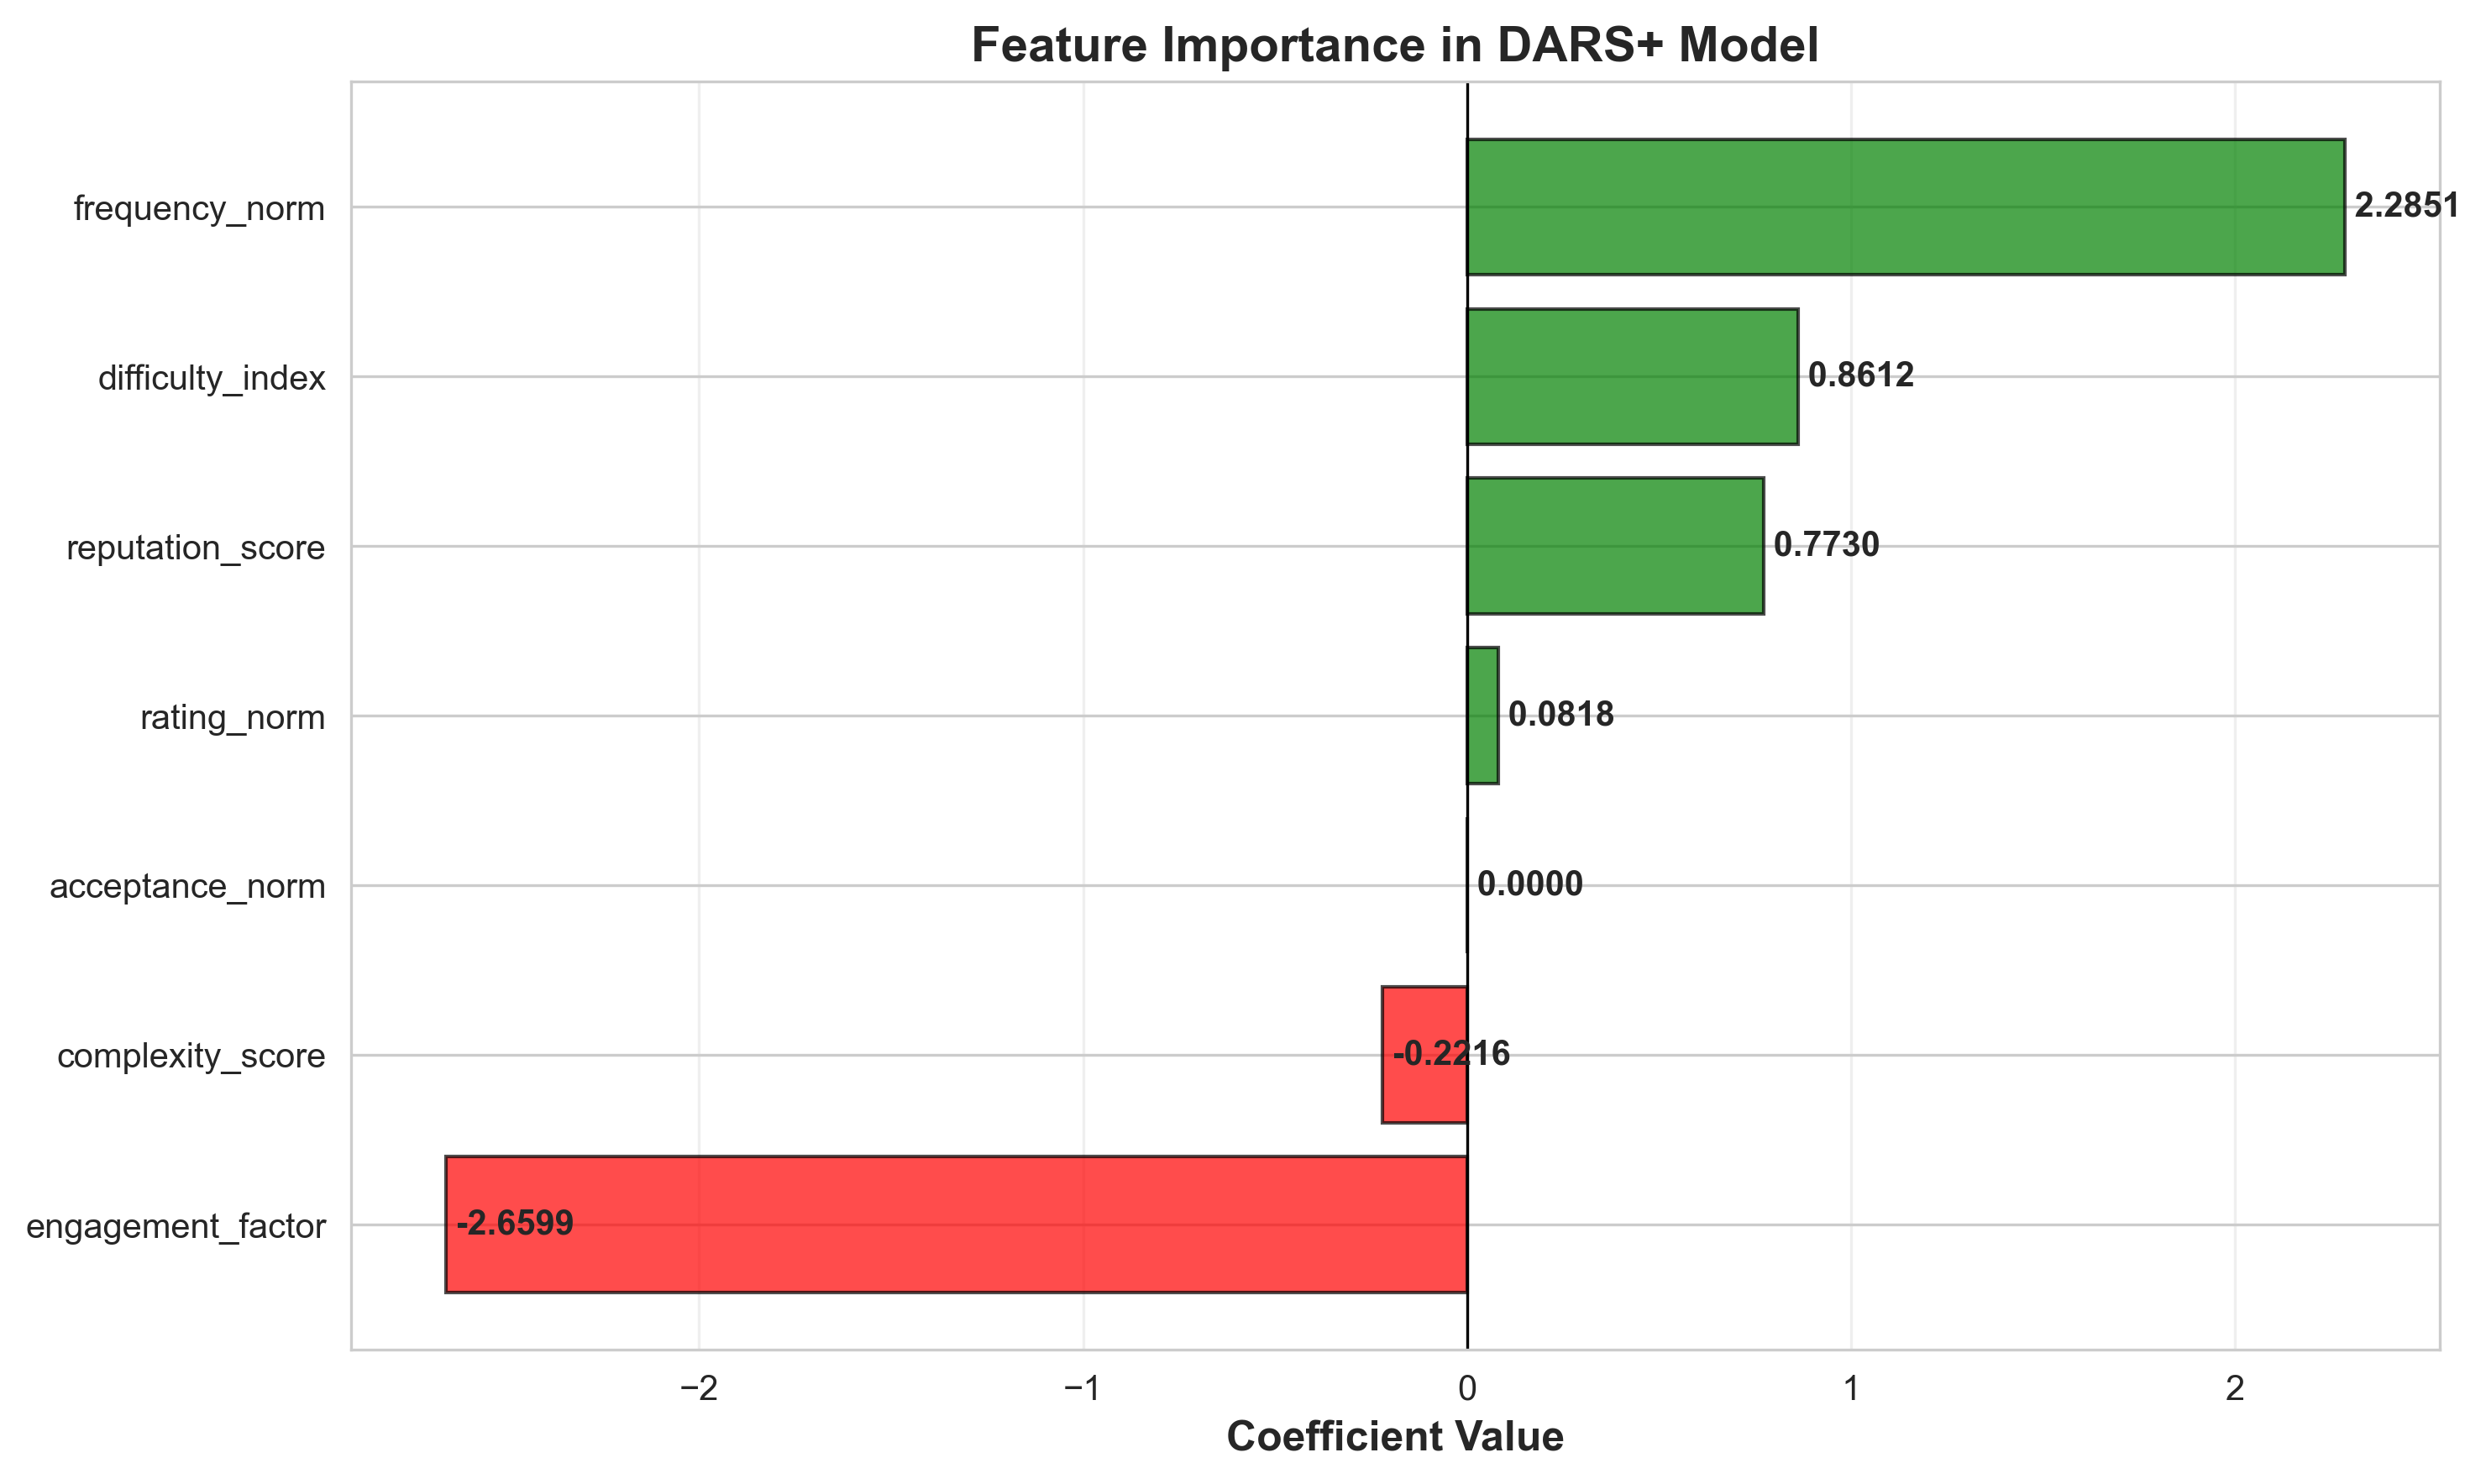
\includegraphics[width=0.45\textwidth]{feature_importance.png}
\caption{Feature importance (logistic regression coefficients). Frequency (+2.29) and difficulty index (+0.86) strongly predict difficulty; engagement factor (-2.66) shows inverse relationship.}
\label{fig:leetcode_features}
\end{figure}

\begin{figure}[t]
\centering
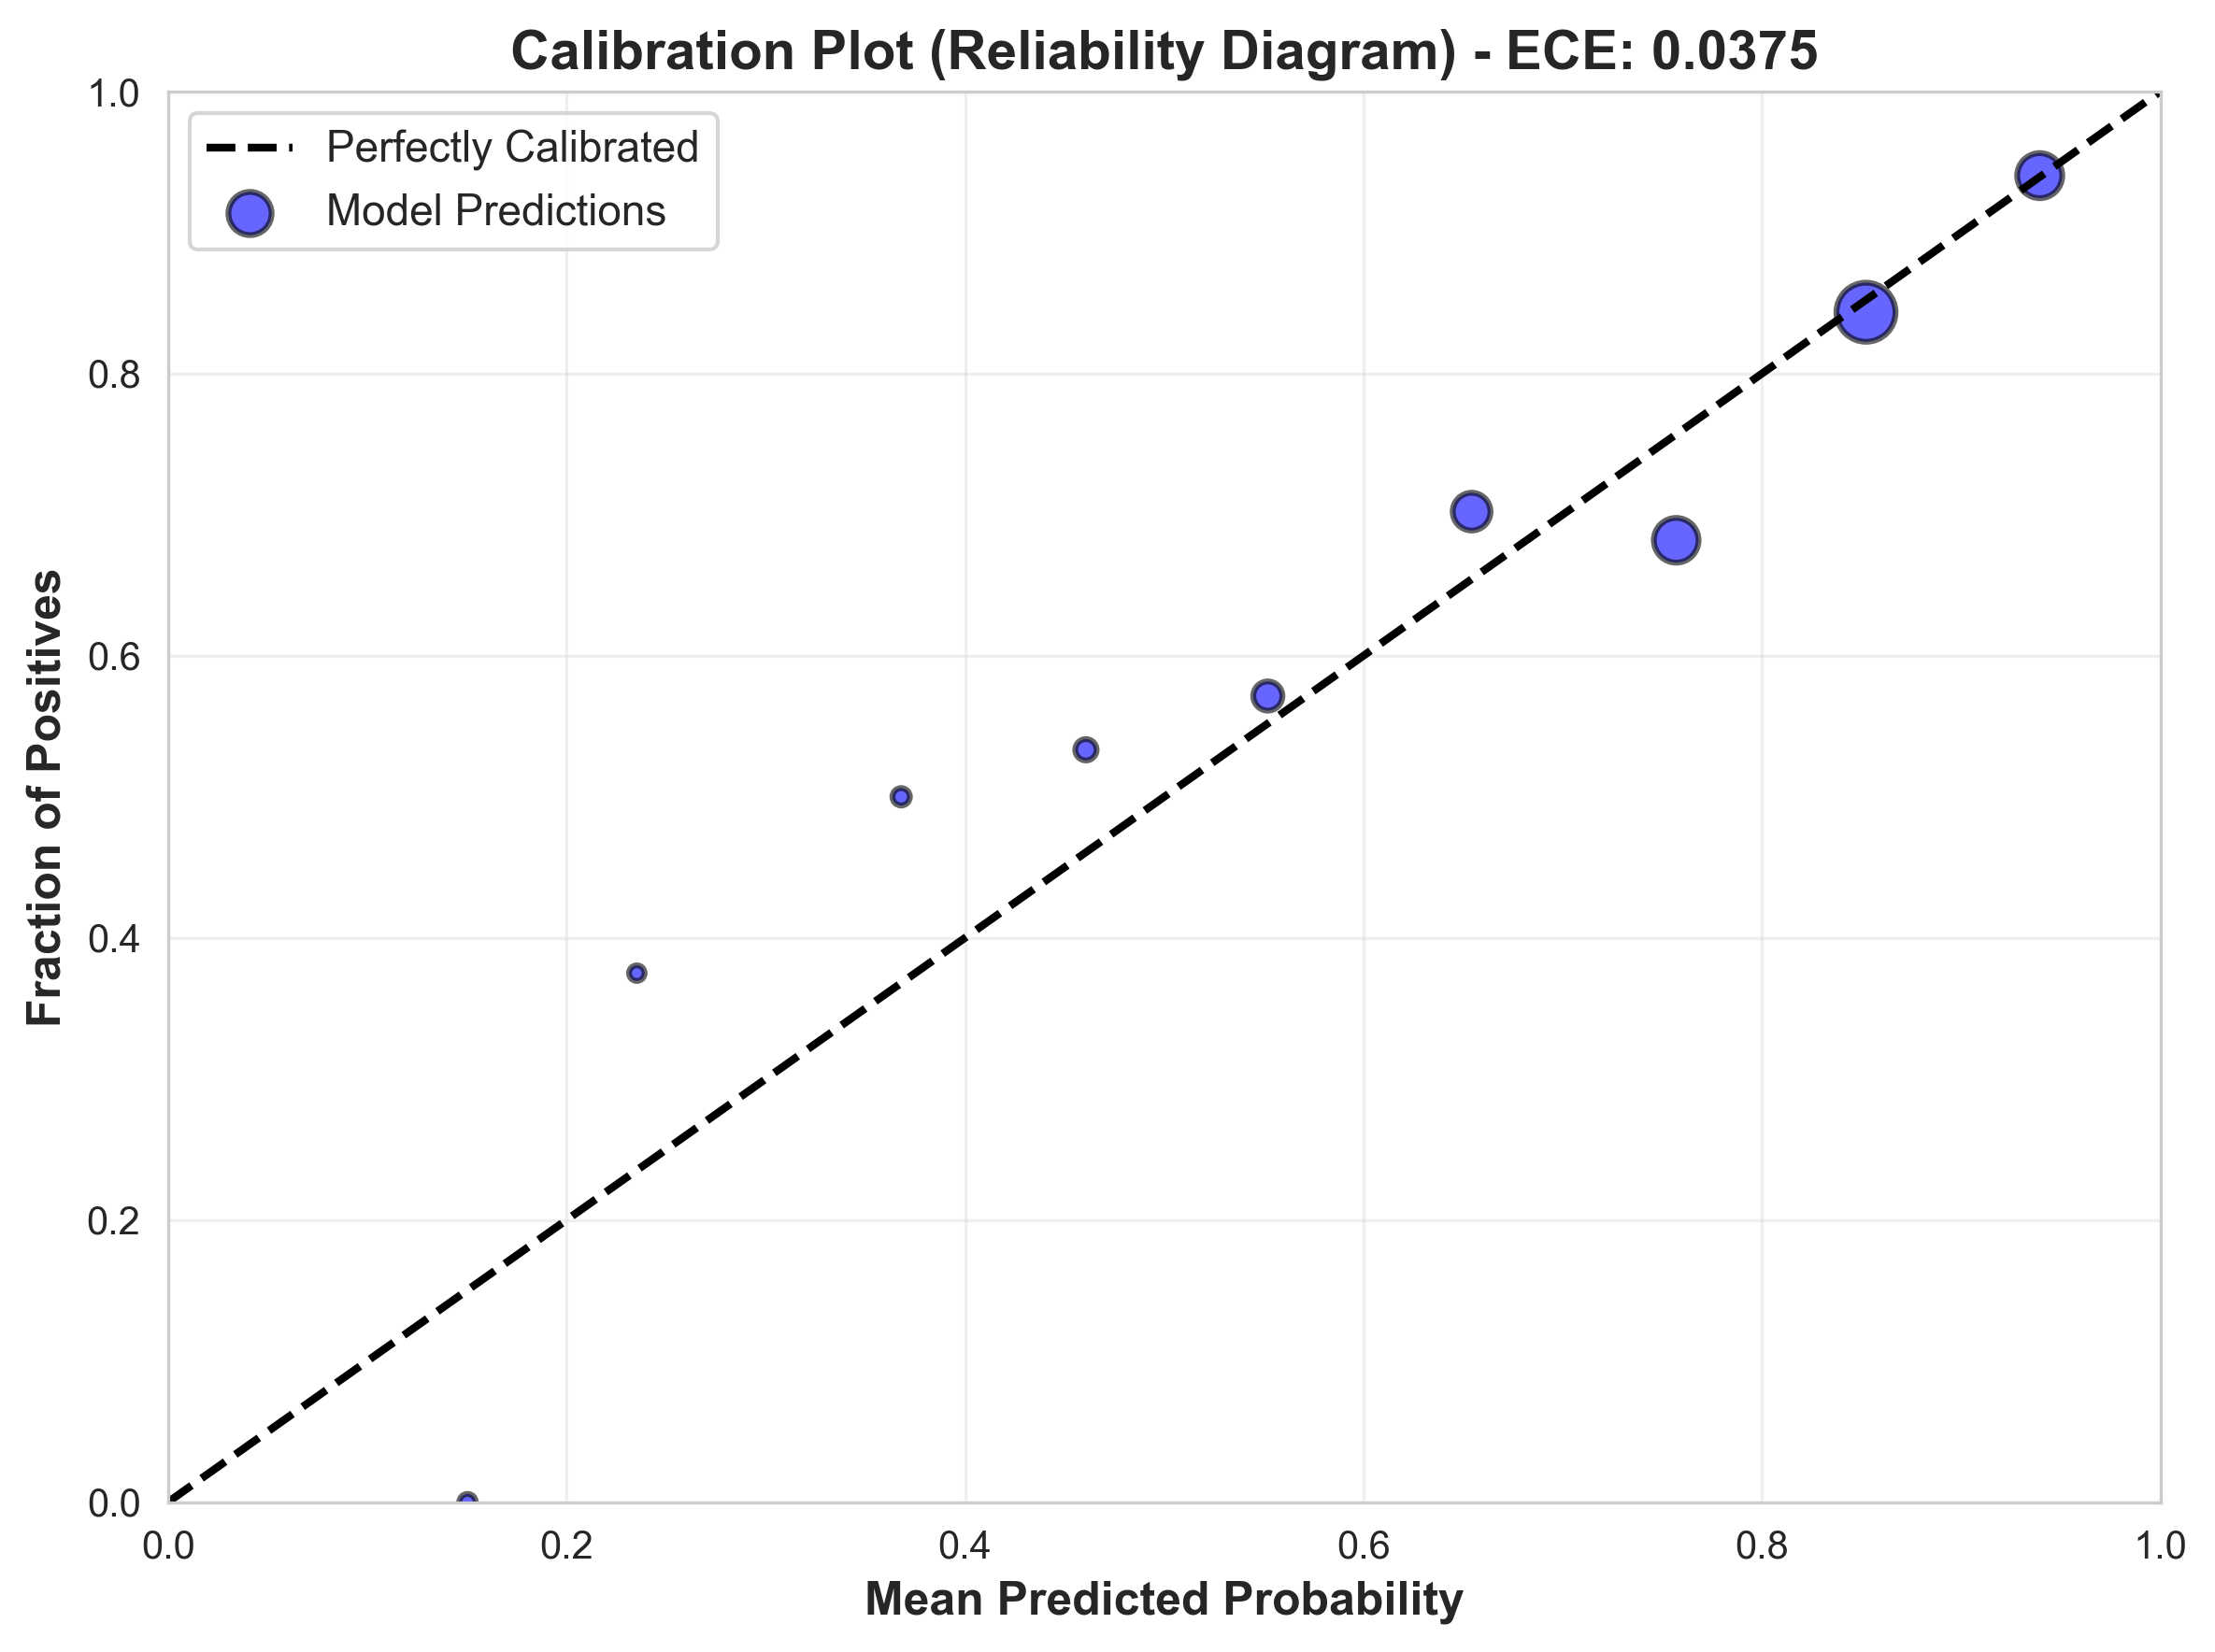
\includegraphics[width=0.45\textwidth]{calibration_plot.png}
\caption{Calibration plot (reliability diagram). Points lie near the diagonal, indicating excellent agreement between predicted and observed difficulty. ECE = 0.0375.}
\label{fig:leetcode_calibration}
\end{figure}

\begin{figure}[t]
\centering
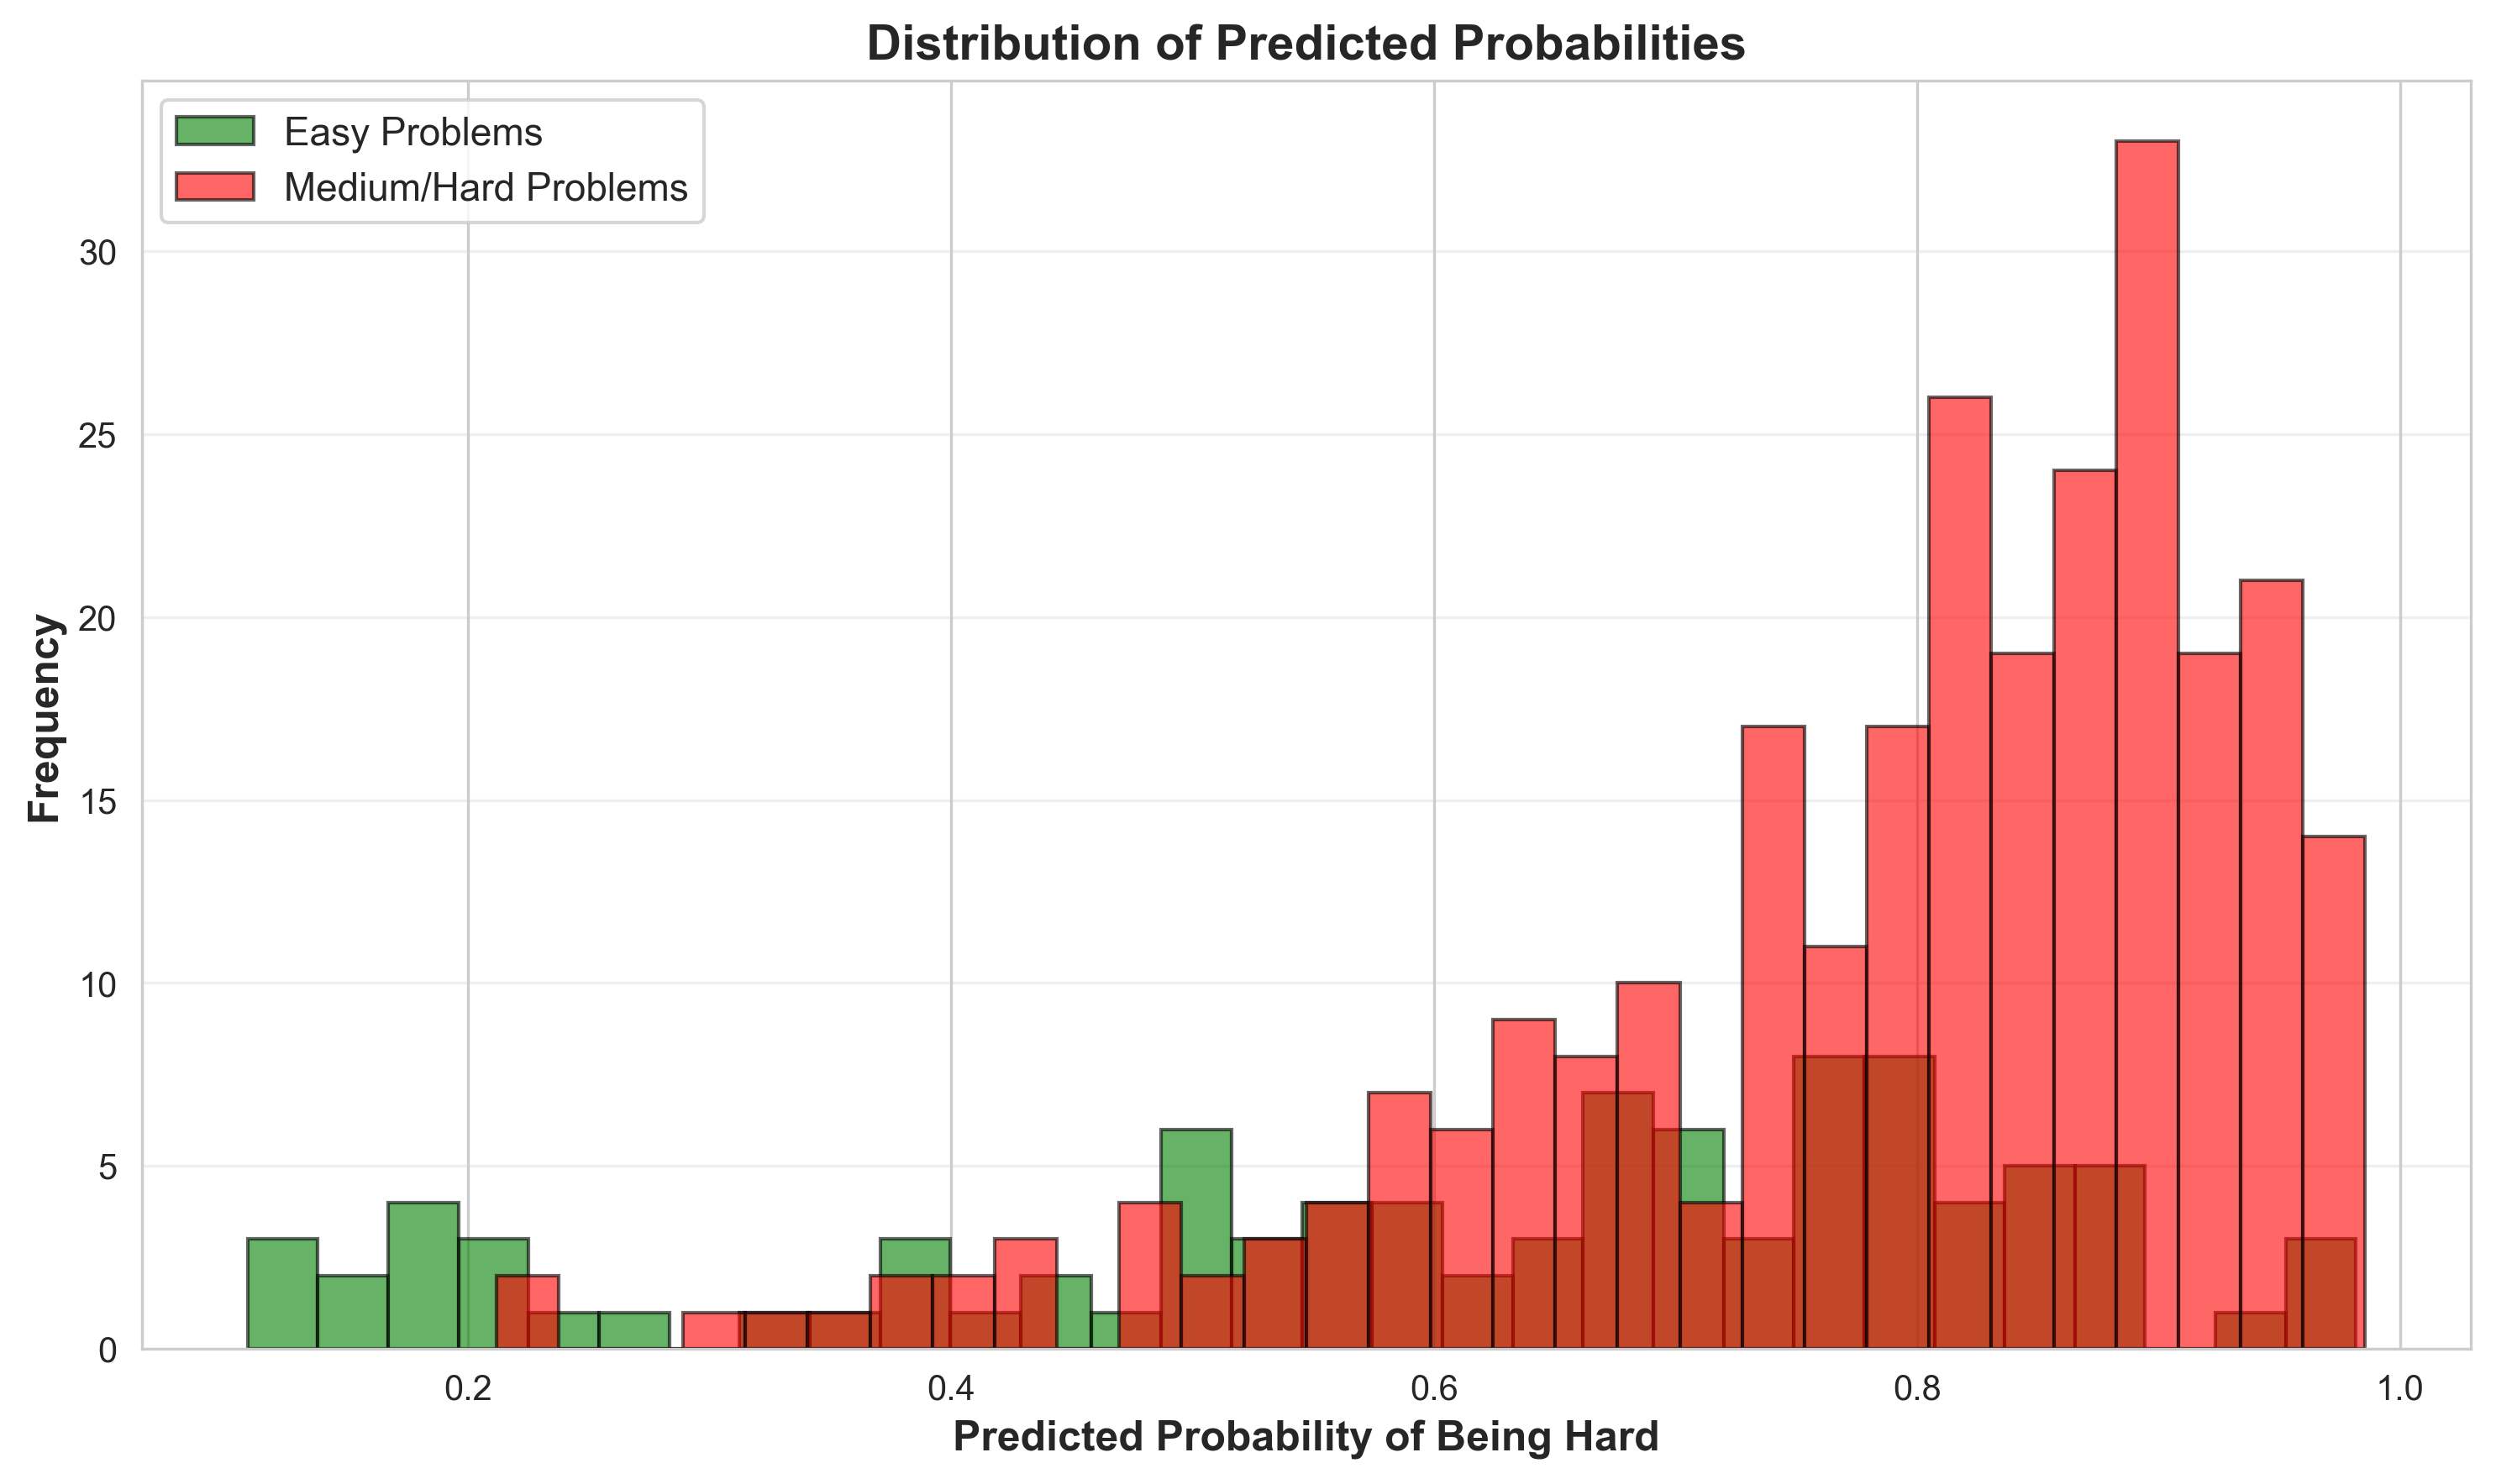
\includegraphics[width=0.45\textwidth]{probability_distribution.png}
\caption{Distribution of predicted probabilities. Green histogram (Easy problems) and red histogram (Medium/Hard problems) show clear separation, validating model discrimination.}
\label{fig:leetcode_probdist}
\end{figure}

\begin{figure}[t]
\centering
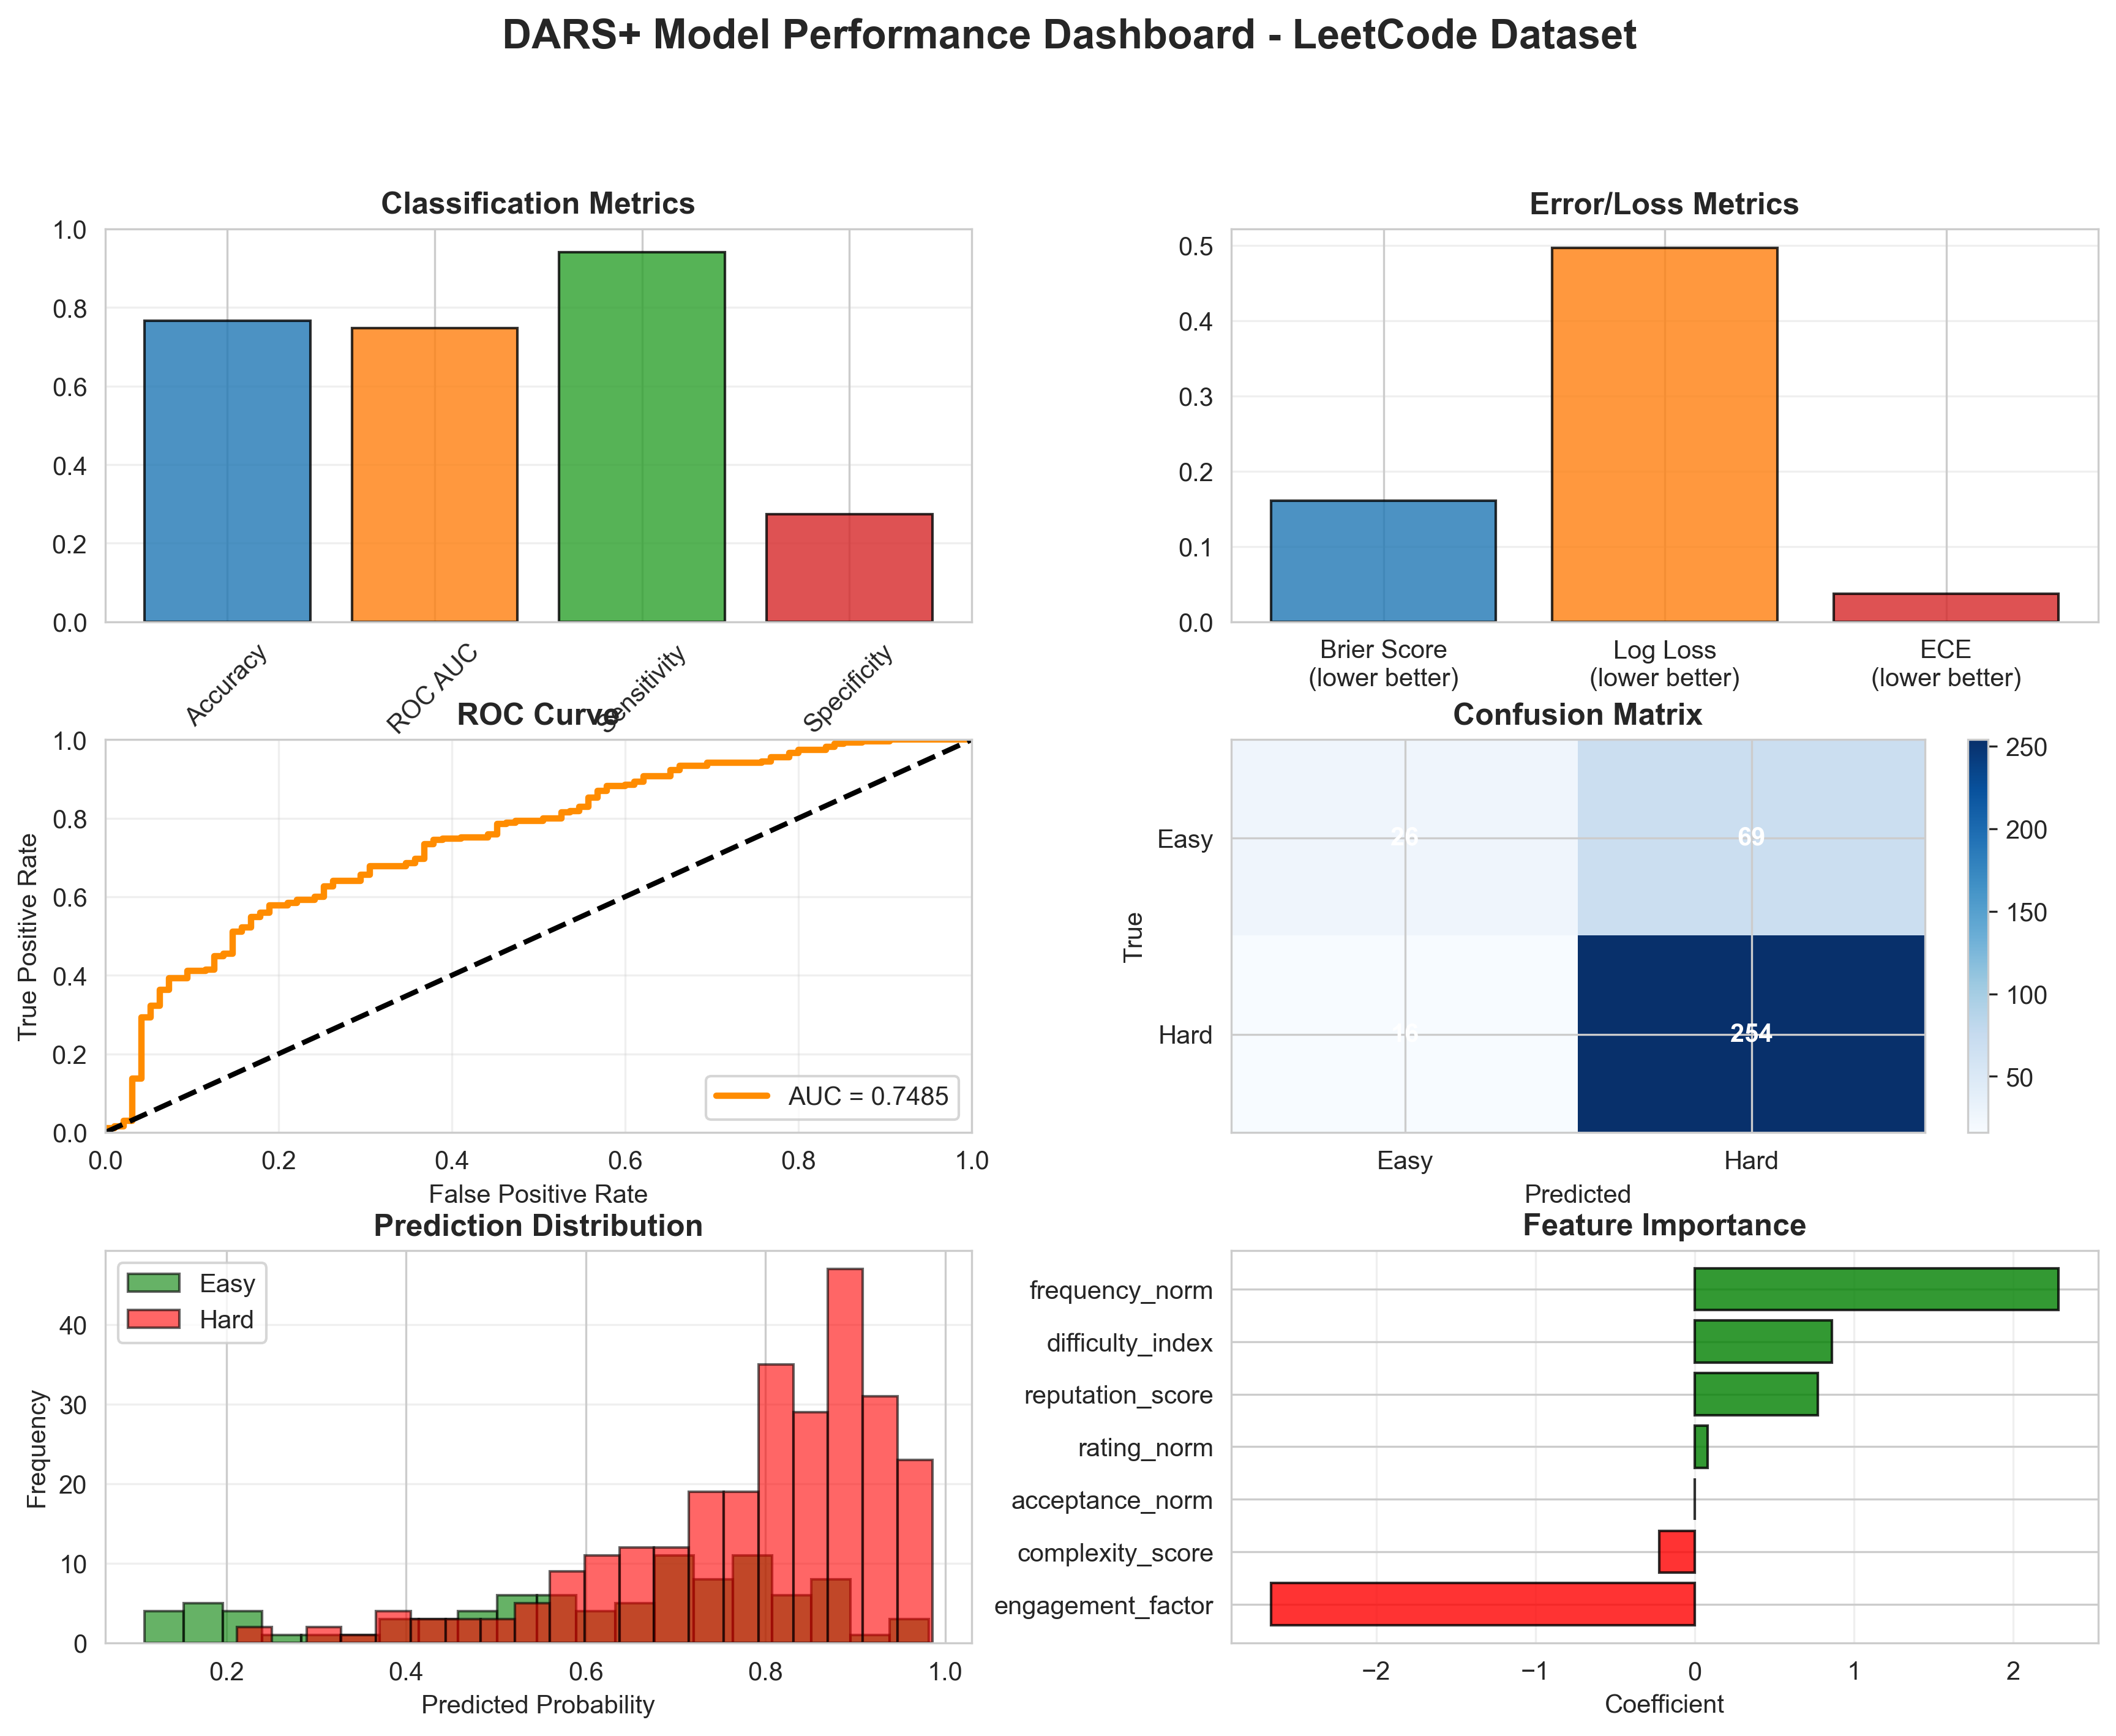
\includegraphics[width=0.45\textwidth]{performance_dashboard.png}
\caption{Comprehensive performance dashboard including metrics, ROC curve, confusion matrix, calibration, and feature importance.}
\label{fig:leetcode_dashboard}
\end{figure}

\section{Limitations}
This study evaluates difficulty prediction from problem metadata, not from per-learner interaction logs. LeetCode's acceptance rates aggregate millions of solvers, providing strong signals but lacking fine-grained learner ability information. The analysis is cross-sectional (snapshot of 1,825 problems) rather than longitudinal. New problems with scarce acceptance-rate data remain challenging (cold-start), as evidenced by Q4 (low acceptance quartile) performance degradation. The fairness analysis reveals substantial bias toward predicting problems as hard due to class imbalance; mitigation strategies (cost-sensitive learning, threshold optimization) should be explored in future deployments.

\section{Future Work}
This paper focuses on problem difficulty prediction using static features and baseline machine learning methods. Future directions include: (1) integrating per-learner interaction logs if available (e.g., from company LeetCode premium accounts), enabling online learning and learner-specific predictions; (2) extending graph neural approaches with richer topologies (problem similarity networks, prerequisite DAGs); (3) developing fairness-aware training procedures that enforce equal TPR across difficulty levels; (4) testing approaches on related platforms (CodeSignal, HackerEarth) for cross-domain generalization; (5) deploying DARS in a live coding platform to measure whether difficulty estimates improve learner outcomes, engagement, and time-to-mastery.

\section{Conclusion}
This paper demonstrated that interpretable feature engineering and dynamic rating mechanisms can achieve accurate and well-calibrated problem difficulty prediction on LeetCode, a massive real-world coding assessment platform. DARS achieves 76.71\% accuracy and 0.7485 ROC AUC while remaining fully interpretable and deployable. Systematic evaluation of six baselines (Elo, Glicko-2, BKT, DKT, SAKT, GNKT) and four graph strategies (skill-only, temporal, expert, hybrid) provides guidance for practitioners choosing assessment models. Fairness analysis reveals actionable insights: category-specific calibration varies, cold-start difficulty (low acceptance rate) degrades performance, and the model exhibits bias toward hard predictions requiring mitigation in deployment. Overall, the results demonstrate that combining problem-level metadata with principled machine learning provides a practical foundation for personalized coding assessment.

\section*{Acknowledgment}
The author thanks the LeetCode community for providing open access to problem metadata and the millions of learners whose aggregated acceptance-rate data enables this research.

\begin{thebibliography}{00}
\bibitem{corbett1994bkt}
A. T. Corbett and J. R. Anderson, ``Knowledge tracing: Modeling the acquisition of procedural knowledge,'' \textit{User Modeling and User-Adapted Interaction}, vol. 4, no. 4, pp. 253--278, 1994.

\bibitem{piech2015dkt}
C. Piech, J. Spencer, J. Huang, S. Ganguli, M. Sahami, L. Guibas, and J. Sohl-Dickstein, ``Deep knowledge tracing,'' in \textit{Proc. 28th Conf. Neural Information Processing Systems (NIPS)}, 2015, pp. 505--513.

\bibitem{pandey2019sakt}
S. Pandey and G. Karypis, ``A self-attentive model for knowledge tracing,'' in \textit{Proc. 12th Int. Conf. Educational Data Mining (EDM)}, 2019, pp. 384--389.

\bibitem{yang2021gikt}
Y. Yang, J. Shen, Y. Qu, Y. Liu, K. Wang, Y. Zhu, W. Zhang, and Y. Yu, ``GIKT: A graph-based interaction model for knowledge tracing,'' in \textit{Proc. European Conf. Machine Learning and Principles and Practice of Knowledge Discovery in Databases (ECML PKDD)}, 2021, pp. 299--315.

\bibitem{elo}
A. E. Elo, \textit{The Rating of Chessplayers, Past and Present}. New York, NY, USA: Arco, 1978.

\bibitem{glickman2008glicko2}
M. E. Glickman, ``Rating systems for all sports,'' \textit{Journal of Quantitative Analysis in Sports}, vol. 4, no. 3, 2008.

\bibitem{barocas2019fairness}
S. Barocas, M. Hardt, and A. Narayanan, \textit{Fairness and Machine Learning}. Berkeley, CA: Draft version, 2019. [Online]. Available: \url{https://fairmlbook.org}

\bibitem{leetcode2023}
LeetCode, ``Online coding platform,'' 2023. [Online]. Available: \url{https://www.leetcode.com/}

\end{thebibliography}

\end{document}
